\PassOptionsToPackage{unicode}{hyperref}
\documentclass[aspectratio=1610, professionalfonts, 9pt, t]{beamer}

\usefonttheme[onlymath]{serif}
\usetheme[showtotalframes]{tudo}


\usepackage{polyglossia}
\setmainlanguage{english}

% Mathematik
\usepackage{multicol}
\usepackage{graphicx}
\usepackage{amssymb}
\usepackage{amsmath}
\usepackage{mathtools}
\usepackage[
  math-style=ISO,
  bold-style=ISO,
  sans-style=italic,
  nabla=upright,
  partial=upright,
]{unicode-math}
\setmathfont{Latin Modern Math}
\usepackage{xparse}
\usepackage{braket}
\usepackage{ulem}
\usepackage{units}
\usepackage[locale=DE,separate-uncertainty=true,per-mode=reciprocal,output-decimal-marker={,},]{siunitx}
\usepackage[section]{placeins}
\usepackage{pdflscape}
\usepackage{expl3}
\usepackage{bookmark}
%Komma als Dezimaltrenner in der mathe Umgebung, um in Umgebungen wie [0, 2] ein Leerzeichen nach dem Komma zu erhalten einfach eins setzen
\usepackage{icomma}
\usepackage{cancel}
\usepackage{tikz}
\usepackage{feynman-tikz}
\usepackage{hyperref}
\usepackage{bookmark}
\usepackage{subfigure}
\usepackage{booktabs}
%Literatuverzeichnis
\usepackage[
  backend=biber,
]{biblatex}
%Quellendatenbank
\addbibresource{lit.bib}

%%%%%%%%%%%%%%%%%%%%%%%%%%%%%%%%%%%%%%%%%%%%%%%%%%%%%%%%%%%%%%%%%%%%%%%%%%%%%%%%
%%%%%-------------Hier Titel/Autor/Grafik/Lehrstuhl eintragen--------------%%%%%
%%%%%%%%%%%%%%%%%%%%%%%%%%%%%%%%%%%%%%%%%%%%%%%%%%%%%%%%%%%%%%%%%%%%%%%%%%%%%%%%

%Titel:
\title{K-Mesonen und wo sie zu finden sind}
%Autor
\author[F.~Koch]{Fabian Koch}
%Datum der Präsentation
\date{02.05.19}
%Lehrstuhl/Fakultät
\institute[Fakultät Physik ]{Fakultät Physik}

\begin{document}

\AtBeginSection[]
{
  \begin{frame}{Inhalt}
    \tableofcontents[currentsection]
  \end{frame}
}


\maketitle

\begin{frame}
  \frametitle{Übersicht}
  \tableofcontents
\end{frame}


\section{Was sind Kaonen}
  \begin{frame}{Was sind Kaonen?}
    \begin{columns}[onlytextwidth]
      \begin{column}{0.4\textwidth}
        \begin{figure}[ht]
          \begin{center}
            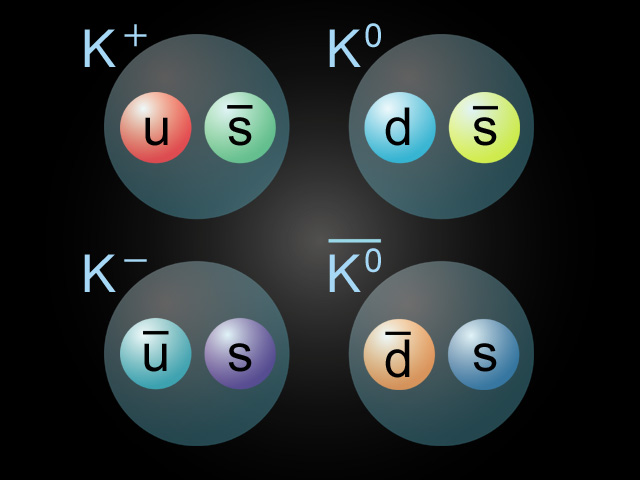
\includegraphics[height=0.6\textheight]{Images/Kaonen.png}
            \caption{Übersicht über die Kaonen}
          \end{center}
        \end{figure}
      \end{column}
      \begin{column}{0.5\textwidth}
        Kaonen:
        \begin{itemize}
          \item sind die leichtesten Teilchen mit Strangeness $S = \pm1$
          \item besitzen einen ganzzahligen Spin
          \item sind Bosonen
          \item verfügen über eine relativ lange Lebensdauer
        \end{itemize}
        \begin{table}
          \centering
          \begin{tabular}{
              S[table-format=6.0]
              S[table-format=3.5]
              @{${}\pm{}$}
              S[table-format=1.5]
              S[table-format=3.4]
              @{${}\pm{}$}
              S[table-format=1.4]
            }
              \toprule
              & \multicolumn{2}{c}{$m \:/\: \si{\mega\electronvolt}$} & \multicolumn{2}{c}{$\tau \:/\: 10^{-10} \si{\second}$} \\
              \midrule
              $K^{\pm}$   & 493.677 & 0.016 & 123.80 & 0.21 \\
              $K⁰_{S}$    & 497.614 & 0.024 & 0.8954 & 0.0004 \\
              $K⁰_{L}$    & 497.614 & 0.024 & 511.6  & 2.1 \\
              ${\pi}^{\pm}$ & 139.57018 & 0.00035 & 260.33 & 0.05 \\
              \bottomrule
          \end{tabular}
        \end{table}
      \end{column}
    \end{columns}
  \end{frame}

\section{Historische Kaonenexperimente}
  \begin{frame}{Weltkarte}
    \begin{figure}[ht]
      \begin{center}
        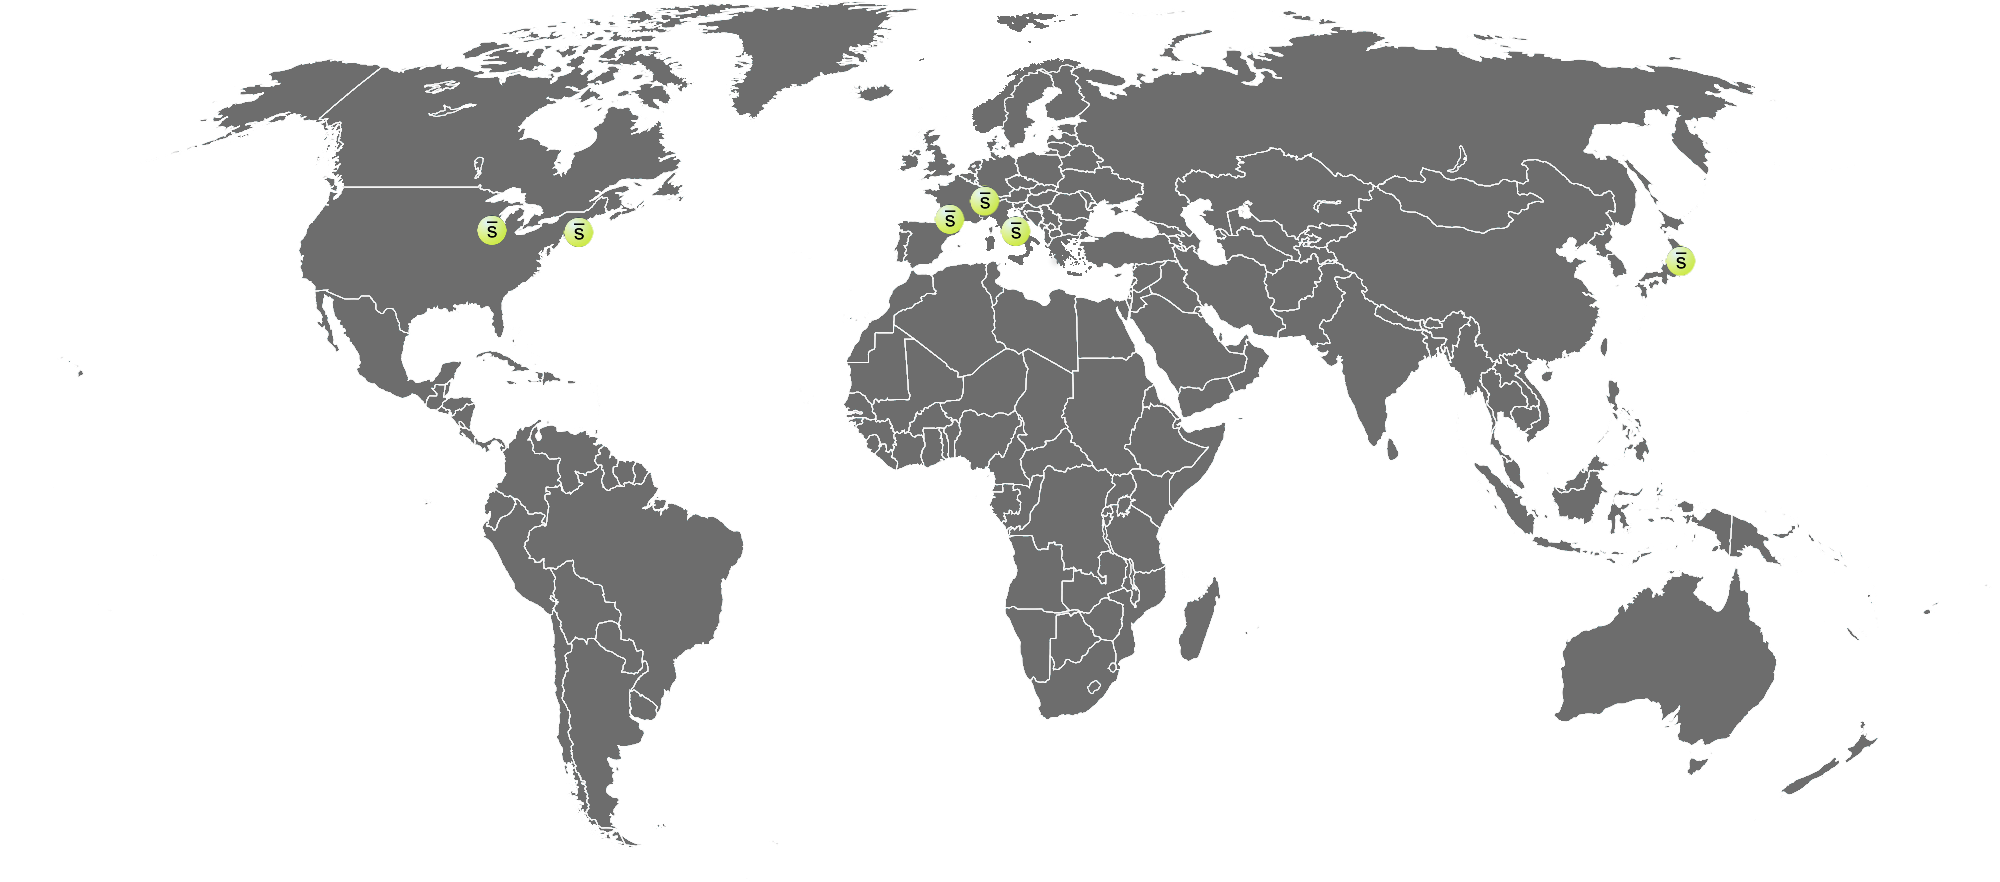
\includegraphics[width=\textwidth]{Images/worldmap.png}
      \end{center}
    \end{figure}
  \end{frame}

\subsection{Entdeckung der Kaonen}

  \begin{frame}{Entdeckung der Kaonen}
    \begin{columns}[onlytextwidth]
      \begin{column}{0.4\textwidth}
        \begin{figure}[ht]
          \begin{center}
            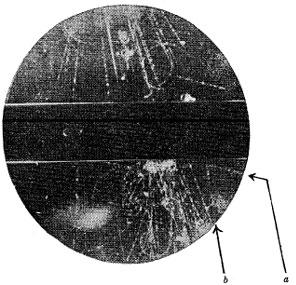
\includegraphics[height=0.6\textheight]{Images/Kaondiscovery.png}
            \caption{Nebelkammeraufnahme der kosmischen Höhenstrahlung von Rochester und Butler 1947}
          \end{center}
        \end{figure}
      \end{column}
      \begin{column}{0.5\textwidth}
        \begin{itemize}
          \item Entdeckung des ersten (neutralen) Kaons 1947 durch George Rochester et. al
          \item Höhenstrahlung wurde in Nebelkammer untersucht
          \item Zerfall eines neutralen Teilchens in ein positives und negatives Pion
          \begin{equation*}
            K^{0} \rightarrow \pi^{+} \pi^{-}
          \end{equation*}
          \item Entdeckung des positiv geladenen Kaons 1949 durch Powell in Kernreaktionen
          \item Zerfall eines positiven Kaons in zwei positive und ein negatives Pion
          \begin{equation*}
            K^{+} \rightarrow \pi^{+} \pi^{+} \pi^{-}
          \end{equation*}
        \end{itemize}
      \end{column}
    \end{columns}
  \end{frame}

  \begin{frame}{Seltsam lange Lebensdauer}
    \begin{columns}[onlytextwidth]
      \begin{column}{0.4\textwidth}
        \begin{figure}[ht]
          \begin{center}
            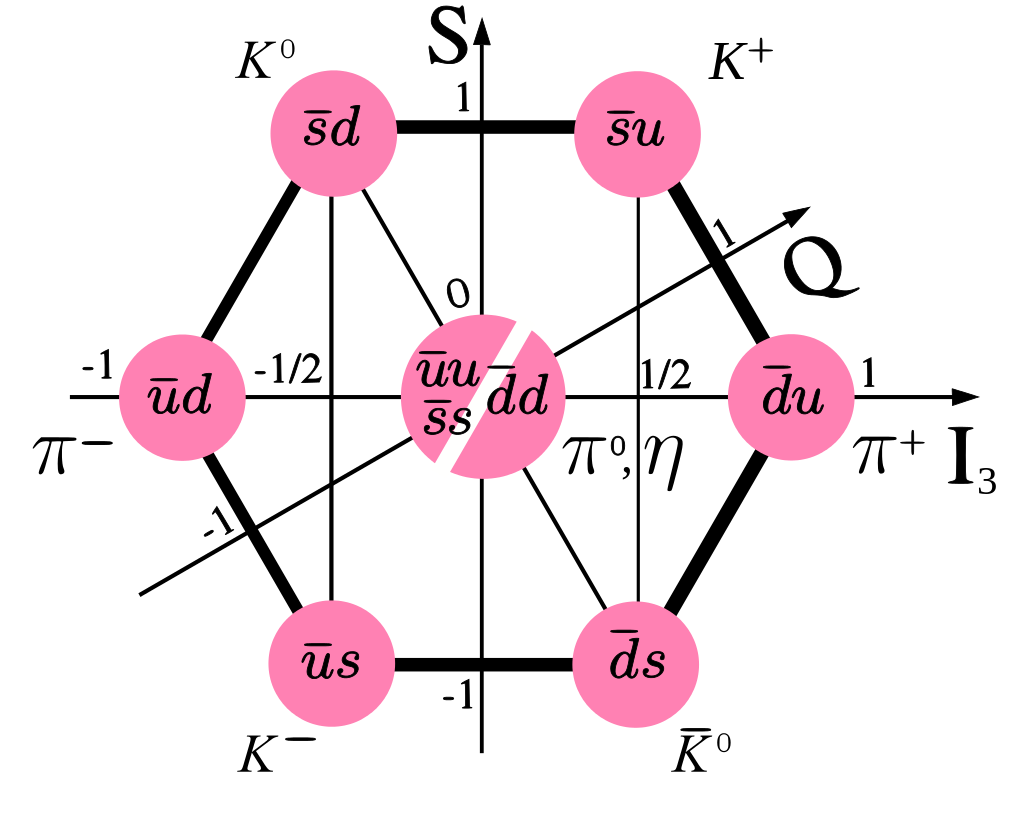
\includegraphics[height=0.6\textheight]{Images/Meson-octet.png}
            \caption{Der achtfache Weg von Gell-Mann und Ne'eman}
          \end{center}
        \end{figure}
      \end{column}
      \begin{column}{0.5\textwidth}
        \begin{itemize}
          \item Sehr leichte Erzeugung (durch starke WW)
          \item Große Halbwertszeit $10^{-10}\si{\second}$ (durch schwache WW)
          \item Gell-Mann 1953: Einführung einer neuen Teilcheneigenschaft/ Quantenzahl \item[\rightarrow] Strangeness
          \item Zerfall leicht möglich, wenn \textbf{S} durch alle Kräfte verletzt wäre
          \item[Aber:] Zerfall nur über die flavourändernde schwache WW möglich
        \end{itemize}
      \end{column}
    \end{columns}
  \end{frame}

\subsection{Paritätsverletzung}

  \begin{frame}{Paritätsverletzung und das Cosmotron}
    \begin{columns}[onlytextwidth]
      \begin{column}{0.4\textwidth}
        \begin{figure}[ht]
          \begin{center}
            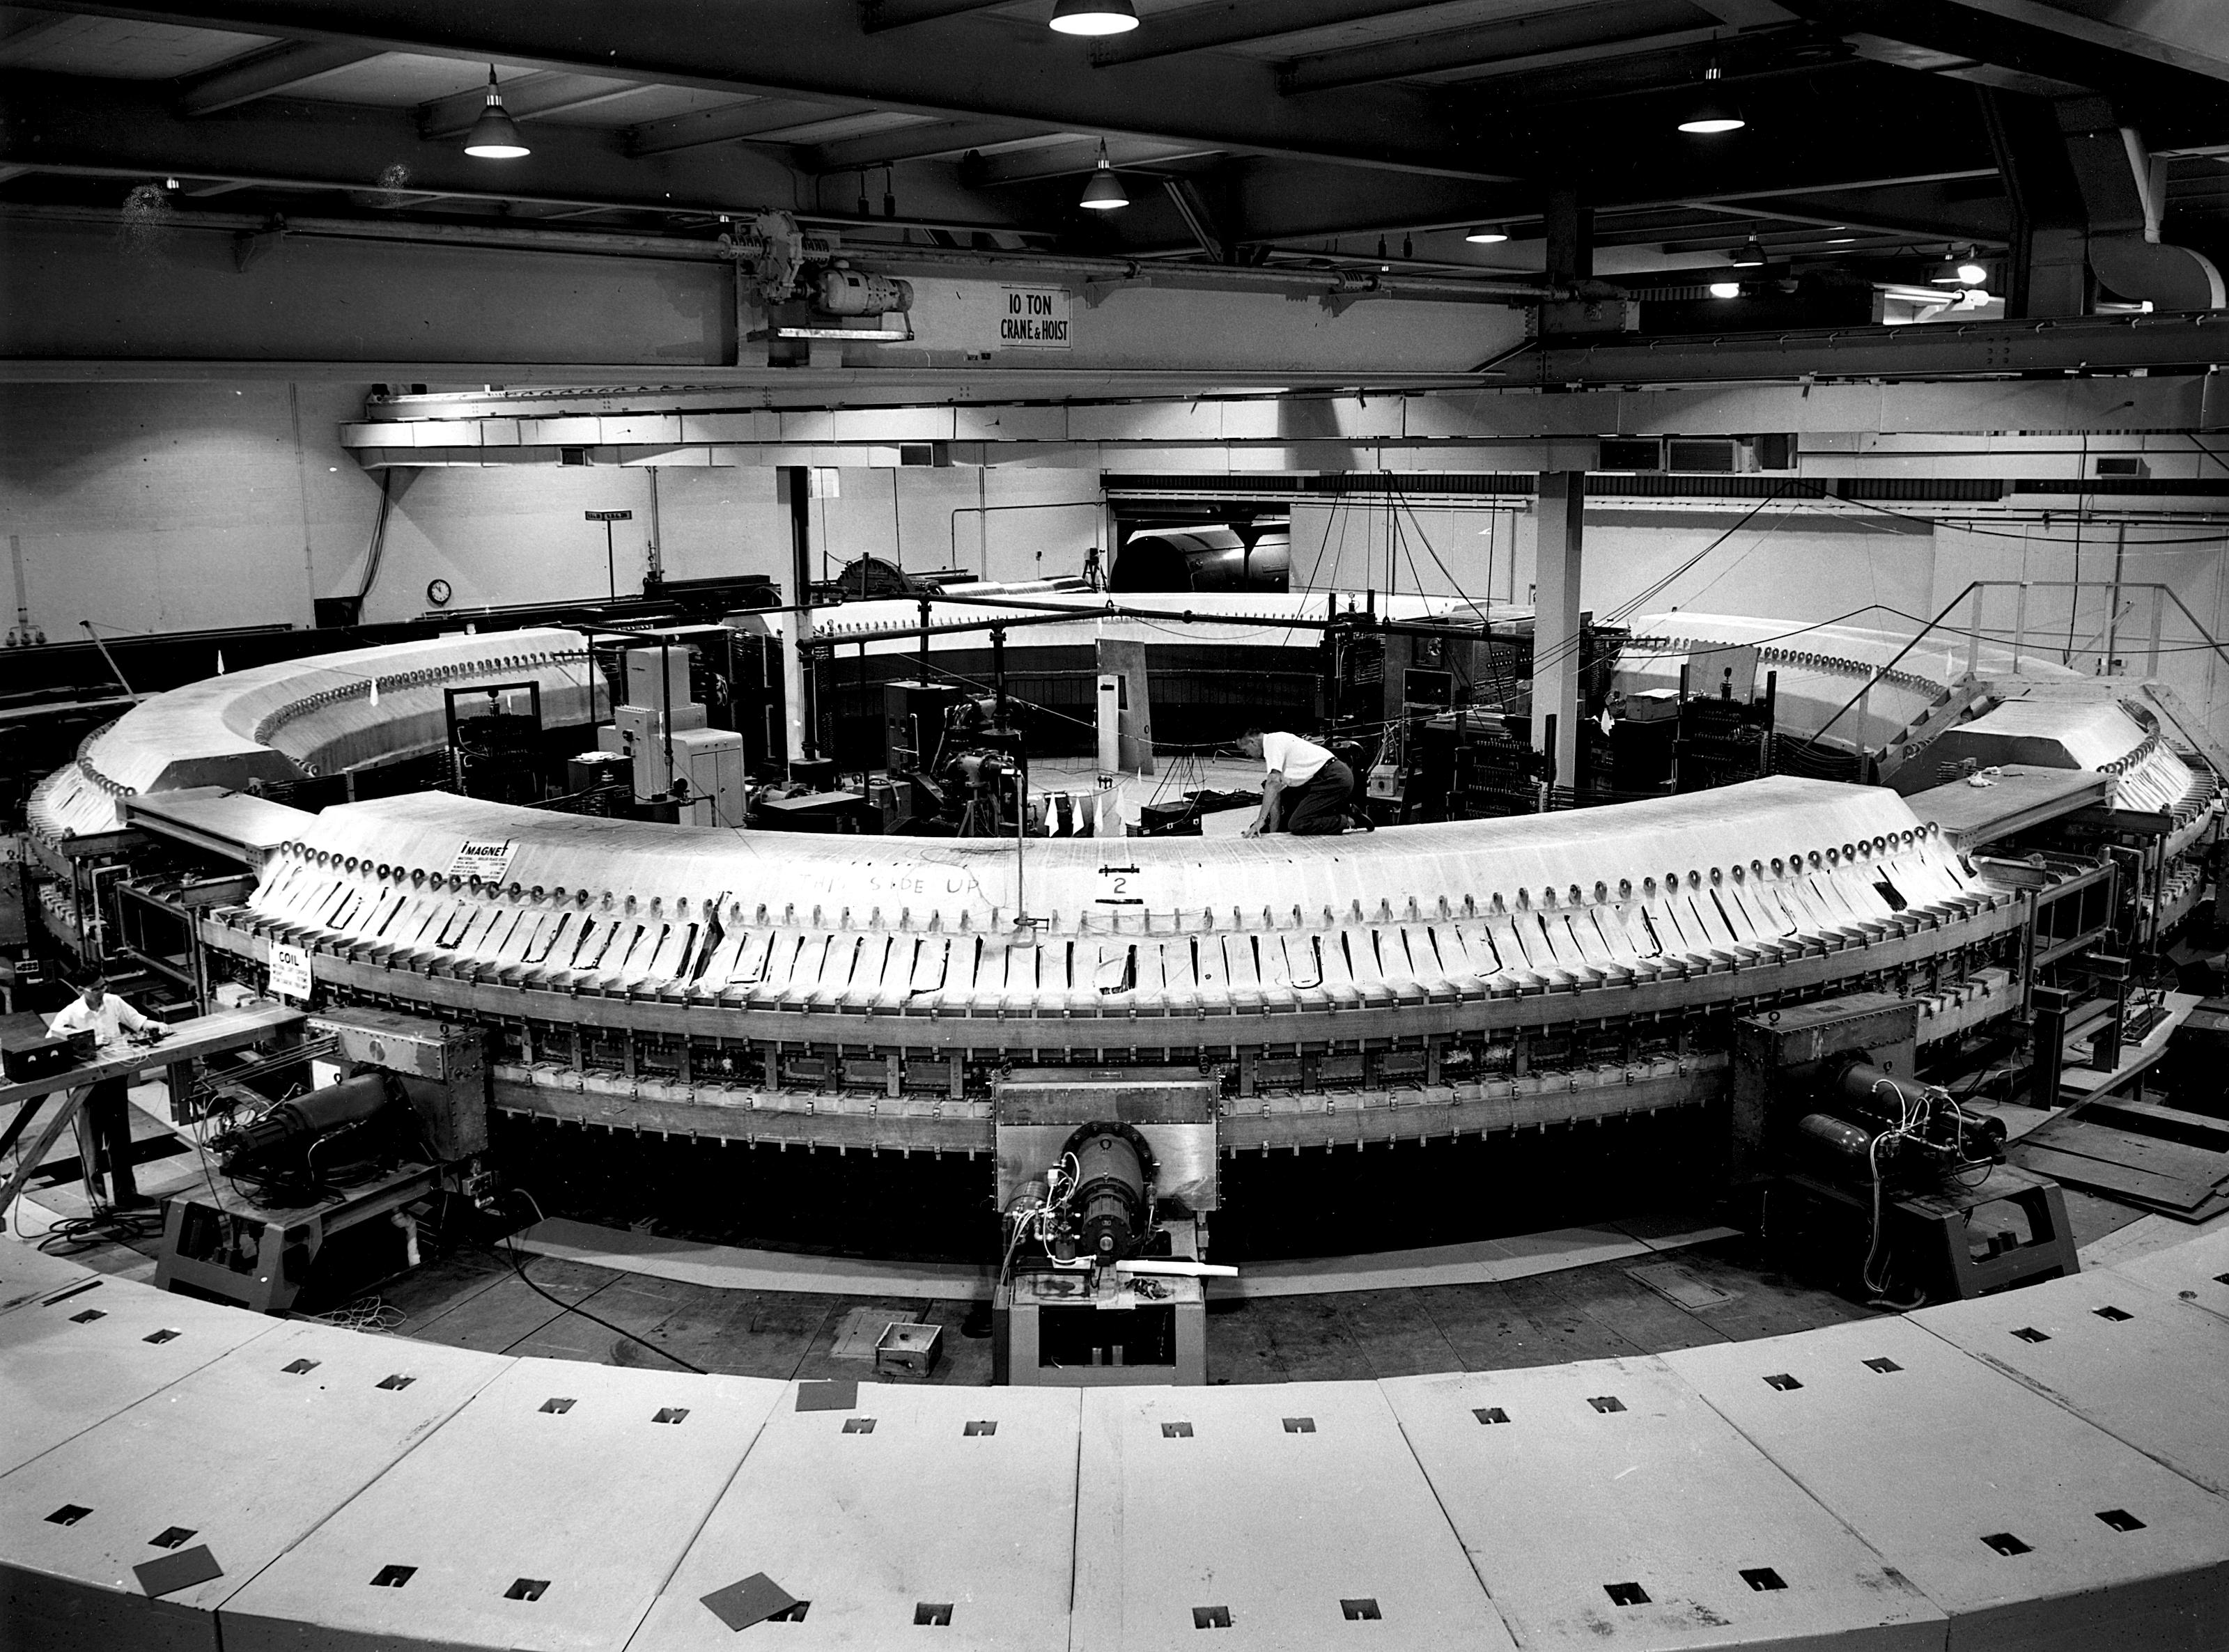
\includegraphics[height=0.6\textheight]{Images/cosmotron.jpg}
            \caption{Das Cosmotron am Brookhaven National Laboratory (1952-1966)}
          \end{center}
        \end{figure}
      \end{column}
      \begin{column}{0.5\textwidth}
        \begin{itemize}
          \item Leistungsstärkstes Proton-Synchrotron (1952) mit Strahlenergien von $\SI{3.3}{\giga\electronvolt}$
          \item Erstmalige Produktion von Mesonen und leichten Hadronen im Labor
          \item Entdeckung $K_{L}$ durch Lande (1956) %in Nebelkammer
          \item Beobachtung der Zerfälle
          \begin{align*}
            \tau^{+} \rightarrow \pi^{+} \pi^{+} \pi^{-} \\
            \theta^{+} \rightarrow \pi^{+} \pi^{0}
          \end{align*}
          \item[] durch T.D. Lee und C.N.Yang (1956)
          \item $\tau^{+}$ und $\theta^{+}$ tatsächlich $K^{+}$
          \item[\rightarrow] Zerfälle verletzen die Paritätserhaltung
        \end{itemize}
      \end{column}
    \end{columns}
  \end{frame}

\subsection{Kaonenmischung}

  \begin{frame}{Long und short? Die Mischung neutraler Kaonen}
    \begin{columns}[onlytextwidth]
      \begin{column}{0.4\textwidth}
        \begin{figure}[ht]
          \feynmandiagram[layered layout, horizontal=a to b, scale=0.9]{
            i1 [particle=\(d\)]
              -- [fermion] a
              -- [photon, edge label=\(W^{-}\)] b
              -- [fermion] f1 [particle=\(s\)],
            i2 [particle=\(\overline s\)]
              -- [anti fermion] c
              -- [photon, edge label'=\(W^{-}\)] d
              -- [anti fermion] f2 [particle=\(\overline d\)],
            { [same layer] a -- [fermion, edge label'=\(u\, c\, t\)] c },
            { [same layer] b -- [anti fermion, edge label=\(u\, c\, t\)] d}
          };
        \end{figure}
        \begin{figure}[ht]
          \feynmandiagram[layered layout, horizontal=a to b, scale=0.9]{
            i1 [particle=\(d\)]
              -- [fermion] a
              -- [fermion, edge label=\(u\, c\, t\)] b
              -- [fermion] f1 [particle=\(s\)],
            i2 [particle=\(\overline s\)]
              -- [anti fermion] c
              -- [anti fermion, edge label'=\(u\, c\, t\)] d
              -- [anti fermion] f2 [particle=\(\overline d\)],
            { [same layer] a -- [photon, edge label'=\(W^{-}\)] c },
            { [same layer] b -- [photon, edge label=\(W^{-}\)] d}
          };
        \end{figure}
      \end{column}
      \begin{column}{0.5\textwidth}
        \begin{itemize}
          \item Flavour-Eigenzustände $\ket{K^{0}}$, $\ket{\overline{K^{0}}}$ unterscheiden sich von den CP-Eigenzuständen:
          \begin{equation*}
            \begin{drcases*}
              CP \ket{K^{0}} = \ket{\overline{K^{0}}} \\
              CP \ket{\overline{K^{0}}} = \ket{K^{0}}
            \end{drcases*}
            \rightarrow
            \begin{cases}
              \ket{K_1} = \frac{1}{\sqrt{2}}\left(\ket{K^{0}} + \ket{\overline{K^{0}}} \right) \\
              \ket{K_2} = \frac{1}{\sqrt{2}}\left(\ket{K^{0}} - \ket{\overline{K^{0}}} \right)
            \end{cases}
          \end{equation*}
          \item $\ket{K_{1}}$ haben CP = +1 und $\ket{K_{2}}$ habe CP = -1
          \item Dabei ist $\ket{K_1} \approx \ket{K_{S}}$ und $\ket{K_2} \approx \ket{K_{L}}$
          \begin{equation*}
            \tau(\ket{K_{L}}) \approx 600 \times \tau(\ket{K_{S}})
          \end{equation*}
          \item Unterschied vor allem in Zerfallsmoden:
          \begin{align*}
            \ket{K_{S}} &\rightarrow \pi^{+} \pi^{-} \\ %Mehr Möglichkeiten im Phasenraum
            \ket{K_{L}} &\rightarrow \pi^{+} \pi^{-} \pi^{0} %Eigentlich verboten, s.h. später
          \end{align*}
        \end{itemize}
      \end{column}
    \end{columns}
  \end{frame}

\subsection{Direkte und indirekte CP-Verletzung}

  \begin{frame}{CP-Verletzung}
    \begin{columns}[onlytextwidth]
      \begin{column}{0.4\textwidth}
        \begin{figure}[ht]
          \begin{center}
            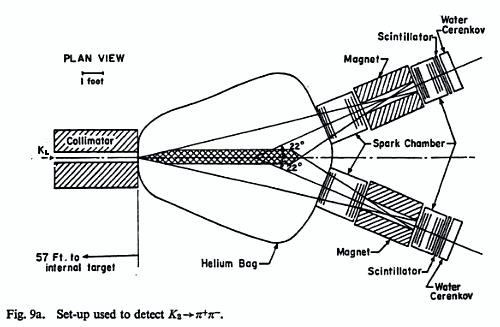
\includegraphics[height=0.6\textheight]{Images/croninfitch_b.png}
            \caption{Das Cronin-Fitch-Experiment am Brookhaven National Laboratory (1964)}
          \end{center}
        \end{figure}
      \end{column}
      \begin{column}{0.5\textwidth}
        \begin{itemize}
          \item Planung 1964 durch Christenson, Cronin, Fitch und Turlay am Brookhaven National Laboratory %Collimator => Bündelung de Teilchenstrahlen
          \item $\SI{17}{\metre}$ lange Beamline
          \item[\rightarrow] Zerfall der $\ket{K_{S}}$
          \item Messung des Winkels $\theta$ zwischen $K_{L}^{0}$-Strahl und Teilchenimpulsen
          \item Bestimmung der Winkelsumme bei 'gleichzeitiger' Detektion
          \item Für Dreikörperzerfall mit großer Wahrscheinlichkeit $\neq 0$
          \item Für Zweikörperzerfälle hingegen mit großer Wahrscheinlichkeit $= 0$
        \end{itemize}
      \end{column}
    \end{columns}
  \end{frame}

  \begin{frame}{Ergebnis}
    \begin{columns}[onlytextwidth]
      \begin{column}{0.4\textwidth}
        \begin{figure}[ht]
          \begin{center}
            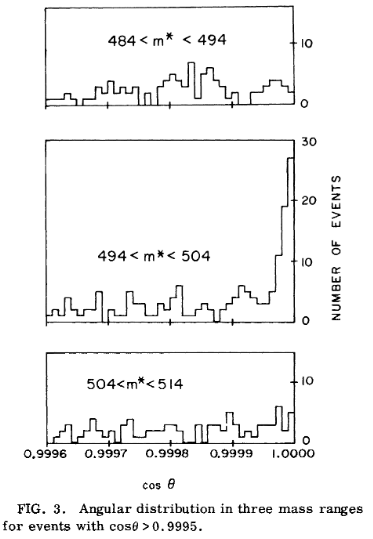
\includegraphics[height=0.8\textheight]{Images/croninfitch_erg.png}
            \caption{Ergebnis der Winkelmessung}
          \end{center}
        \end{figure}
      \end{column}
      \begin{column}{0.5\textwidth}
        \newline
        \newline
        \newline
        \newline
        Tatsächlich wurde der Zerfall
        \begin{align*}
          K_{L} \rightarrow \pi^{+} \pi^{-}
        \end{align*}
        gemessen.
      \end{column}
    \end{columns}
  \end{frame}

  \begin{frame}{Wie kann das sein?}
    \begin{itemize}
      \item Konsequenz: $\ket{K_{S}}$ und $\Ket{K_{L}}$ keine reinen CP- Eigenzustände
      \item[\rightarrow] Beide Zustände enthalten kleine Teile des anderen Zustands:
    \end{itemize}
    \begin{columns}[onlytextwidth]
      \begin{column}{0.5\textwidth}
        \begin{align*}
          \ket{K_{L}^0} &= \frac{\epsilon \ket{K_1} + \ket{K_2}}{\sqrt{1 + \epsilon^2}} \\
          \ket{K_{S}^0} &= \frac{\ket{K_1} + \epsilon \ket{K_2}}{\sqrt{1 + \epsilon^2}}
        \end{align*}
      \end{column}
      \begin{column}{0.5\textwidth}
        \begin{align*}
          \\
          |\epsilon| = (2.229\pm0.010)\times10^{-3}
        \end{align*}
      \end{column}
    \end{columns}
    \begin{itemize}
      \item Auftreten von CP-Verletzung innerhalb der Oszillation (indirekt) oder eines Zerfalls (direkt)
      \item Problem: Im Jahre 1964 noch keine Quarks oder der CKM-Mechanismus bekannt
      \item Erst 1973: Postulierung der drei Quarkfamilien und des CKM-Mechanismus durch Kobayashi und Maskawa
      \item[\rightarrow] Grundlage für viele weitere Forschungsprogramme
    \end{itemize}
  \end{frame}

  \begin{frame}{Wie wird das gemessen?}
    \begin{columns}[onlytextwidth]
      \begin{column}{0.4\textwidth}
        \begin{align*}
          \eta_{00} = \frac{A \left(K_L \rightarrow \pi^0 \pi^0 \right)}{A \left(K_S \rightarrow \pi^0 \pi^0 \right)} &= \epsilon - 2 \epsilon^{\prime} \\
          \eta_{\pm} = \frac{A \left(K_L \rightarrow \pi^+ \pi^- \right)}{A \left(K_S \rightarrow \pi^+ \pi^- \right)} &= \epsilon +  \epsilon^{\prime}
        \end{align*}
        \begin{equation*}
          \symup{Re}(\epsilon' / \epsilon) = \frac{1}{6} \left\{1 - \left|\frac{\eta_{00}}{\eta_{\pm}}\right|^2 \right\}
        \end{equation*}
      \end{column}
      \begin{column}{0.5\textwidth}
        \begin{itemize}
          \item Messung der unterschiedlichen partiellen Zerfallsbreiten
          \begin{align*}
            \Gamma \left(K_L \rightarrow \pi^0 \pi^0 \right) &\neq \Gamma \left(K_S \rightarrow \pi^0 \pi^0 \right) \\
            \Gamma \left(K_L \rightarrow \pi^+ \pi^- \right) &\neq \Gamma \left(K_S \rightarrow \pi^+ \pi^- \right)
          \end{align*}
          \item[\rightarrow] Bilden der Verhältnisse
          \item[Vorteil:] Viele systematische Fehler kürzen sich
          \item $\epsilon^{\prime} = 0$: keine direkte CP-Verletzung
          \item $\epsilon^{\prime} \neq 0$: direkte CP-Verletzung
          \item Bis in die 90er kein eindeutiges Ergebnis durch Experimente
        \end{itemize}
      \end{column}
    \end{columns}
  \end{frame}

  \section{Moderne Experimente}

  \subsection{Motivation für moderne Kaon-Experimente}

  \begin{frame}{Motivation}
    Warum sind Kaonen-Experimente immer noch wichtig für das Verständnis fundamentaler Fragen der Teilchenphysik?
    \begin{itemize}
      \item Gibt es noch weitere Ursachen für CP-Verletzung, abseits der komplexen Phase der CKM-Matrix?
      \item Inwieweit ist die Leptonuniversalität berücksichtigt?
      \item Wie weit können die Grenzen der Teilchenphysik in Bezug auf seltene Prozesse gebracht werden?
      \item Gibt es neue Physik, die durch die Untersuchung von Pinguindiagrammen beobachten werden kann?
      \item Können fundamentale Symmetrien, wie CPT, untersucht werden und wenn ja bis zu welchem Grad?
    \end{itemize}
  \end{frame}

  \subsection{Zurück zu direkter CP-Verletzung}

  \begin{frame}{Wer war an der Messung von Re$(\epsilon^{\prime} / \epsilon)$ beteiligt?}
    KTeV am FermiLab
    \begin{itemize}
      \item Kaons at the TeVatron
      \item Vorläufer: E731 $\rightarrow$ Anfang: 198x Abschluss Datenanalyse: 1992
      \item[\rightarrow] Re$(\epsilon^{\prime} / \epsilon) = (7.4\pm5.9) \times10^{-4}$
      \item KTeV $\rightarrow$ Anfang: 1996 Abschluss Datenanalyse: 2011
      \item[\rightarrow] Re$(\epsilon^{\prime} / \epsilon) = (19.2\pm2.1) \times10^{-4}$
    \end{itemize}
    NA48 am Cern
    \begin{itemize}
      \item North Area 48
      \item Vorläufer NA31 $\rightarrow$ Anfang: 1986 Abschluss Datenanalyse: 1993
      \item[\rightarrow] Re$(\epsilon^{\prime} / \epsilon) = (23.0\pm6.5) \times10^{-4}$
      \item NA48 $\rightarrow$ Anfang: 1997 Abschluss Datenanalyse: 2002
      \item[\rightarrow] Re$(\epsilon^{\prime} / \epsilon) = (14.7\pm2.2) \times10^{-4}$
    \end{itemize}
  \end{frame}

  \subsection{NA48}

  \begin{frame}{Das Experiment NA48}
    \begin{figure}
      
\includegraphics[height=0.8\textheight]{Images/ripcern.png}
    \end{figure}
  \end{frame}

  \begin{frame}
    \begin{columns}[onlytextwidth]
      \begin{column}{0.4\textwidth}
        \begin{figure}[ht]
          \begin{center}
            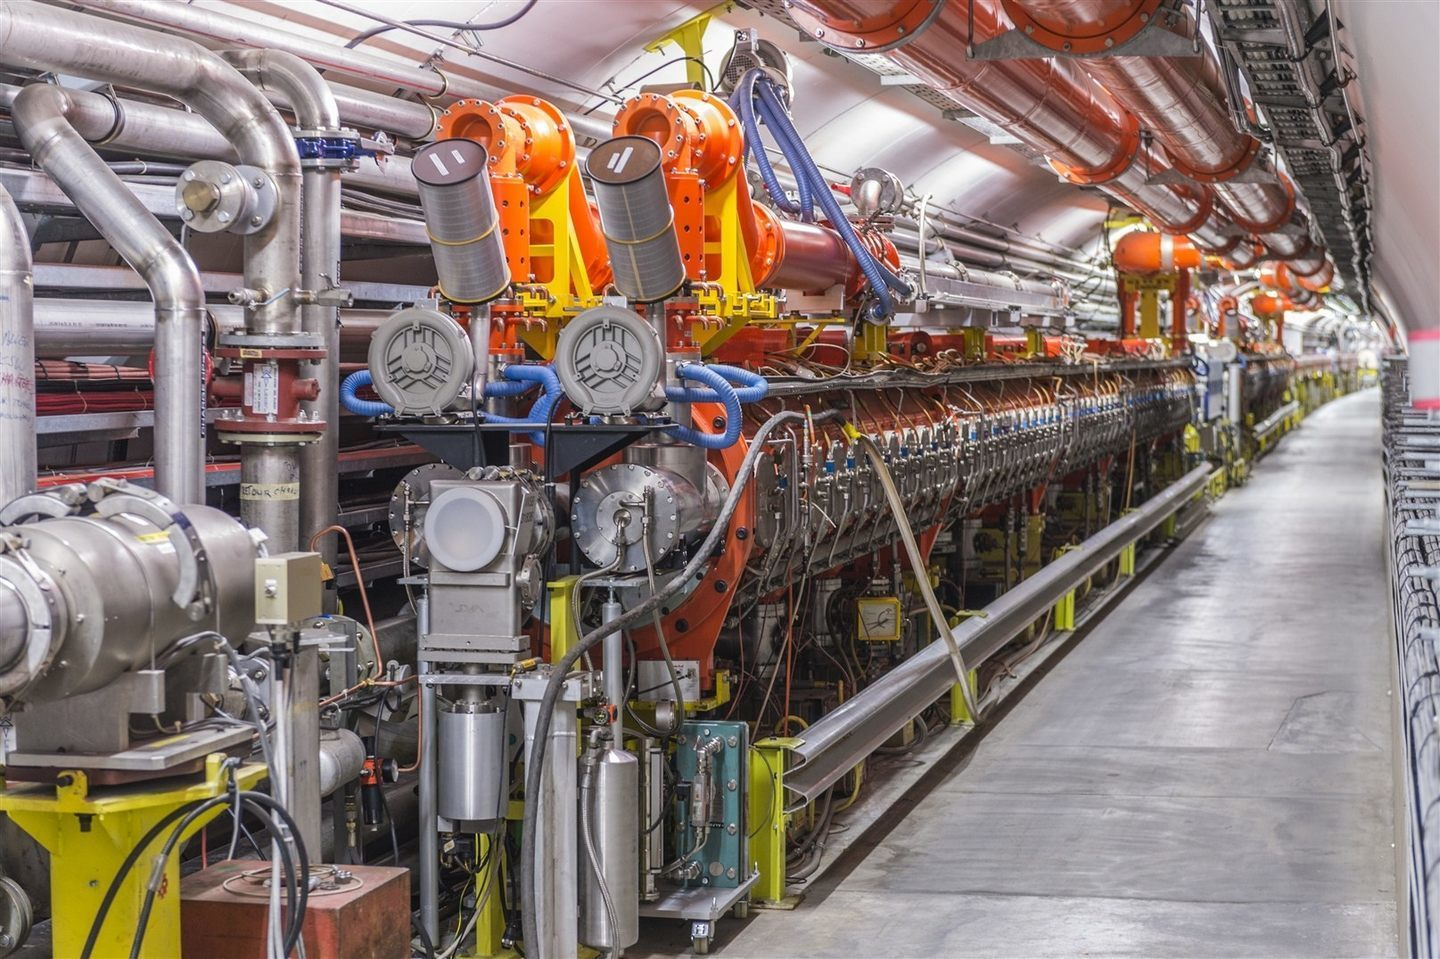
\includegraphics[width=\textwidth]{Images/sps.jpg} %Zuschnippeln
            \caption{Tunnel des Super Proton Synchrotrons (SPS)}
          \end{center}
        \end{figure}
      \end{column}
      \begin{column}{0.5\textwidth}
        \begin{itemize}
          \item Fixed target mit $\SI{450}{\giga\electronvolt}$ vom SPS
          \item Gleichzeitige Messung von $\ket{K_L}$ und $\ket{K_S}$
          \item[\rightarrow] Extraktion von $\epsilon'$ durch Messen des Doppelverhältnisses
          %\item Trennung von $\ket{K_L}$ und $\ket{K_S}$ nach letztem Collimator
          \item[\rightarrow] Aufspalten des Protonstrahles in $\ket{K_L}$ und später $\ket{K_S}$
          \item Auftreffen von $\ket{K_L}$ und $\ket{K_S}$ am gleichen Detektorpunkt
          \item Vertexrekonstruktion ausreichend für Zerfall in $\pi^{\pm}$
          \item[\rightarrow] Problematischer $\pi^0$
        \end{itemize}
      \end{column}
    \end{columns}
  \end{frame}

  \begin{frame}{Aufbau der NA48 Beamline}
    \begin{figure}[ht]
      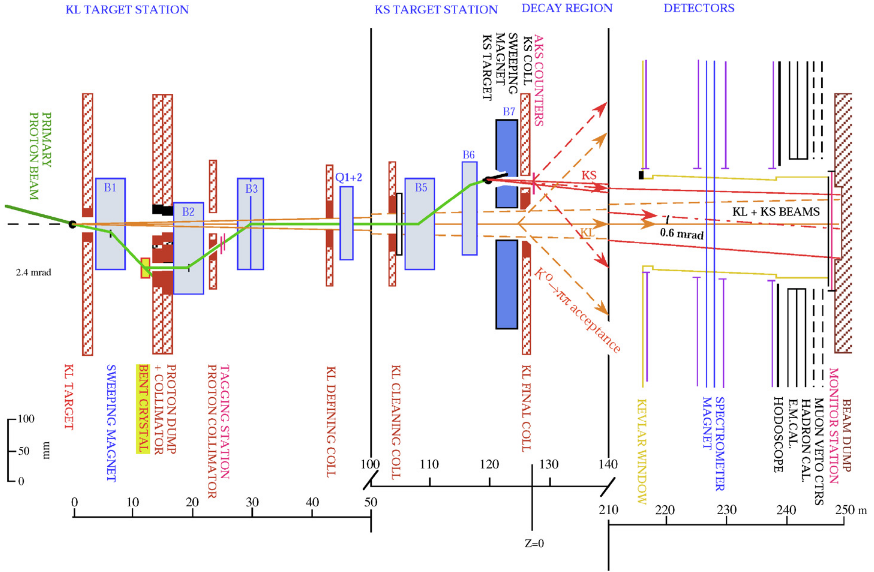
\includegraphics[height=0.95\textheight]{Images/na48quer.png}
      \caption{Beamline des NA48-Experiments}%Stolzr auf bent crystals
    \end{figure}
  \end{frame}

  \begin{frame}
    \begin{columns}[onlytextwidth]
      \begin{column}{0.4\textwidth}
        \begin{figure}[ht]
          \begin{center}
            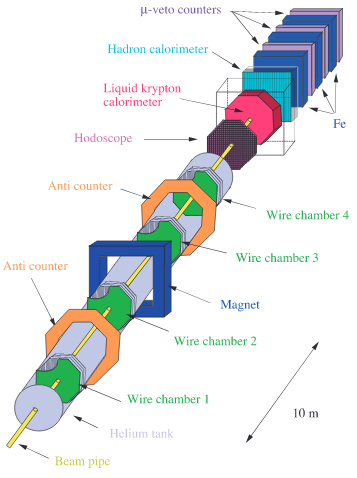
\includegraphics[height=0.8\textheight]{Images/na48detector.png} %Zuschnippeln
            \caption{Detektor des NA48-Experiments}
          \end{center}
        \end{figure}
      \end{column}
      \begin{column}{0.6\textwidth}
        \begin{itemize}
          \item Trennung der Zerfallsprodukte von $\ket{K_L}$ und $\ket{K_S}$
          \item Verhindern von Regeneration ($\ket{K_L} \rightarrow \ket{K_S}$)
          \item Vetomechanismen um andere Zerfälle zu filtern, z.B. Myonkammern
          \item Messung der Produkte:
          \begin{equation*}
            \begin{drcases*}
              K_L \\
              K_S
            \end{drcases*}
            \rightarrow
            \begin{cases}
              \pi^0 \pi^0 \rightarrow \gamma \gamma \gamma \gamma \symup{:EMKalorimeter} \\
              \pi^+ \pi^- \symup{:Spektrometer, Hadronenkalorimeter}
            \end{cases}
          \end{equation*}
          \item[\rightarrow] Besonders bei $\ket{K_S}$ sehr frühe Detektion von $\gamma$ durch AKS

        \end{itemize}
      \end{column}
    \end{columns}
  \end{frame}

  \subsection{KTeV}

  \begin{frame}{Das KTeV-Experiment}
    \begin{figure}
      
\includegraphics[height=0.8\textheight]{Images/rip.png}
    \end{figure}
  \end{frame}

  \begin{frame}
    \begin{columns}[onlytextwidth]
      \begin{column}{0.4\textwidth}
        \begin{figure}[ht]
          \begin{center}
            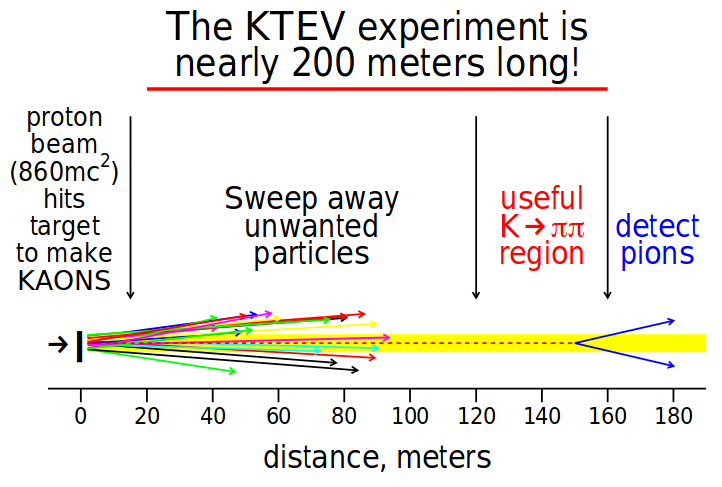
\includegraphics[height=0.6\textheight]{Images/ktevdistance.png} %Zuschnippeln
            \caption{Konzept des KTeV Experiments}
          \end{center}
        \end{figure}
      \end{column}
      \begin{column}{0.5\textwidth}
        \begin{itemize}
          \item Kaonzerfall im Vakuum um Kollision mit Luft zu verhindern
          \begin{align*}
            K^0 &\rightarrow \pi^+ \pi^- \\
                &\rightarrow \pi^0 \pi^0
          \end{align*}
          \item $\pi$-Impulse werden durch die Krümmung ihrer Bahnen gemessen (Magnetfeld)
          \item Anschließend Spurmessung durch 'wire chambers'
          \item $\pi$ die Detektor verfehlen, werden simuliert und berücksichtigt
        \end{itemize}
      \end{column}
    \end{columns}
  \end{frame}

  \begin{frame}
    \begin{figure}[ht]
      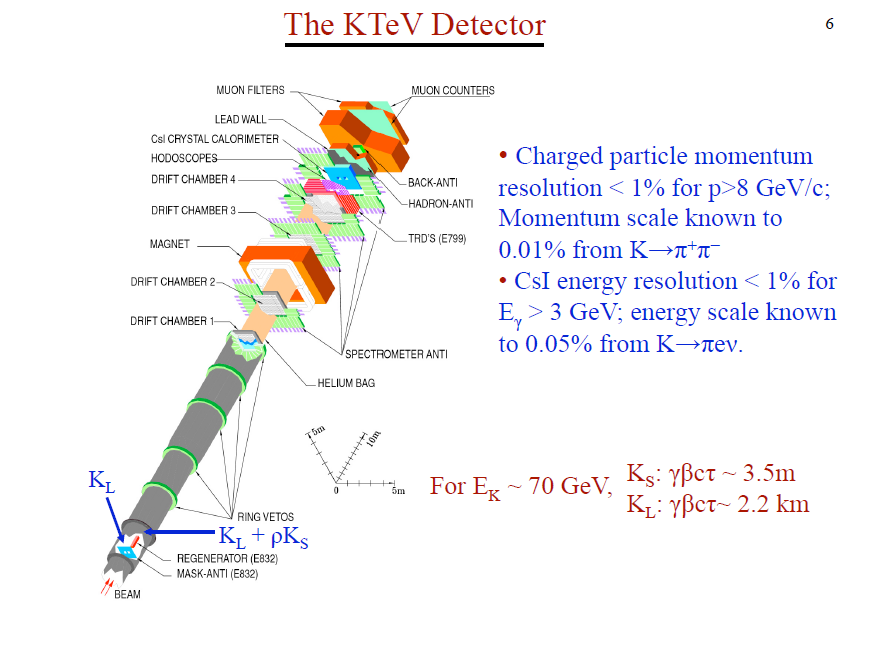
\includegraphics[height=0.8\textheight]{Images/KTEVDETEKTOR.png}
      \caption{Detektor des KTeV-Experiments}
    \end{figure}
  \end{frame}

  \subsection{Ergebnisse von KTeV und NA48}

  \begin{frame}{Ergebnisse beider Experimente}
    \begin{figure}
      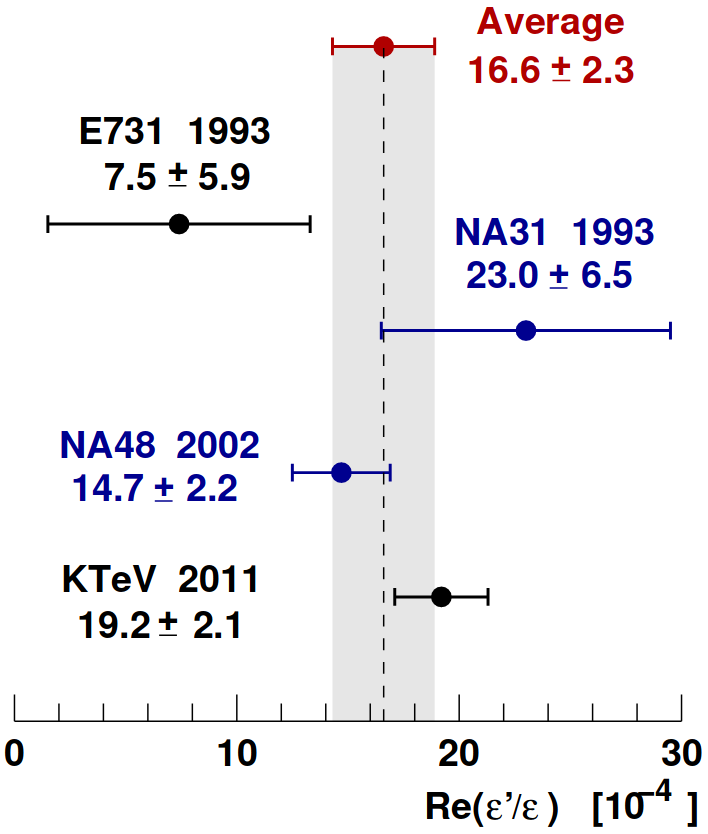
\includegraphics[height=0.9\textheight]{Images/ktevna48.png}
    \end{figure}
  \end{frame}

\section{Seltene Zerfälle und Präzisionsmessungen}

  \subsection{Der goldene Zerfall der Kaonphysik}

  \begin{frame}{Der goldene Zerfall der Kaonphsyik}
    \begin{itemize}
      \item Der Anteil des Zerfalls
      \begin{equation*}
        K \rightarrow \pi \nu \bar{\nu}
      \end{equation*}
      \item[] ist im Standardmodell stark unterdrückt ($<10^{-10}$)
      \item[\rightarrow] Goldener Zerfall der Kaonphsyik
      \item Berechnung aber mit hoher Genauigkeit möglich
      \item[\rightarrow] Hohe Sensitivität auf Prozesse außerhalb des Standardmodells
      \item[\rightarrow] Potentiell auf mehrere Hundert TeV sensitiv
      \item Wichtig um Daten von B-Zerfällen auszuwerten
      \item[\rightarrow] Aufspüren neuer Freiheitsgrade wie Leptoquark %teilchen, die an QUarks und Leptonen koppeln und eine Umwandlung ermöglichen
    \end{itemize}
  \end{frame}

  \begin{frame}{Feynmangraphen}
    \begin{columns}[onlytextwidth]
      \begin{column}{0.3\textwidth}
        \begin{figure}[ht]
          \feynmandiagram[horizontal=a to b, scale=1.1] {
          a -- [anti fermion, edge label=\(\overline q\)] b;
          };
        \end{figure}
        \begin{figure}[ht]
          \vspace*{-0.4cm}
          \feynmandiagram[vertical=e to f,scale = 0.85] {
          a -- [fermion, edge label=\(s\)] b -- [boson, edge label=\(W\)] c -- [fermion, edge label=\(d\)] d,
          b -- [fermion, edge label'=\(t\)] e -- [fermion, edge label'=\(t\)] c,
          e -- [boson, edge label=\(Z\)] f,
          h -- [fermion, edge label=\(\bar{\nu}\)] f -- [fermion, edge label=\(\nu\)] i;
          };
        \end{figure}
      \end{column}
      \begin{column}{0.3\textwidth}
        \begin{figure}[ht]
          \feynmandiagram[horizontal=a to b, scale=1.1] {
          a -- [anti fermion, edge label=\(\overline q\)] b;
          };
        \end{figure}
        \begin{figure}[ht]
          \vspace*{-0.4cm}
          \feynmandiagram[vertical=e to f, scale=0.85] {
          a -- [fermion, edge label=\(s\)] b -- [fermion, edge label=\(t\)] c -- [fermion, edge label=\(d\)] d,
          b -- [boson, edge label'=\(W\)] e -- [boson, edge label'=\(W\)] c,
          e -- [boson, edge label=\(Z\)] f,
          h -- [fermion, edge label=\(\bar{\nu}\)] f -- [fermion, edge label=\(\nu\)] i;
          };
        \end{figure}
      \end{column}
      \begin{column}{0.3\textwidth}
      \begin{figure}[ht]
        \hspace*{0.15cm}
        \feynmandiagram[horizontal=a to b, scale=0.92] {
        a -- [fermion, edge label=\(\overline q\)] b;
        };
      \end{figure}
      \begin{figure}[ht]
        \vspace*{-0.4cm}
        \feynmandiagram[layered layout, vertical=a to b, scale=0.85]{
          i1 [particle=\(d\)]
            -- [fermion] a
            -- [photon, edge label'=\(W\)] b
            -- [fermion] f1 [particle=\(\nu\)],
          i2 [particle=\(s\)]
            -- [anti fermion] c
            -- [photon, edge label'=\(W\)] d
            -- [anti fermion] f2 [particle=\(\overline \nu\)],
          { [same layer] a -- [fermion, edge label'=\(t\)] c },
          { [same layer] b -- [anti fermion, edge label'=\(l\)] d}
          };
        \end{figure}
      \end{column}
    \end{columns}
      \begin{itemize}
        \item[\rightarrow] Nur Pinguin- und Boxdiagramme
        \item[\rightarrow] hohe Sensitivität auf neue Physik
      \end{itemize}
  \end{frame}

  \begin{frame}{Erste Versuche}
    \begin{itemize}
      \item Zerfall $K^+ \rightarrow \pi^+ \nu \bar{\nu}$ durch E787/E949 am BNL untersucht %(Brookhaven National Laboratory)
      \item[\rightarrow] Einschränkung auf:
      \begin{align*}
        \symup{Experiment: BR}(K^+ \rightarrow \pi^+ \nu \bar{\nu}) &< 3.35 \times 10^{-10} @\, \SI{90}{\percent}CL \\
        \symup{Theorie: BR}(K^+ \rightarrow \pi^+ \nu \bar{\nu})     &=  (8.4\pm1.0) \times 10^{-11}
      \end{align*}
      \item Zerfall $K_L \rightarrow \pi^0 \nu \bar{\nu}$ durch E391a am J-PARC/KEK untersucht
      \item[\rightarrow] Einschränkung auf:
      \begin{align*}
        \symup{Experiment: BR}(K^+ \rightarrow \pi^+ \nu \bar{\nu}) &< 2.6 \times 10^{-8} @\, \SI{90}{\percent}CL \\
        \symup{Theorie: BR}(K^+ \rightarrow \pi^+ \nu \bar{\nu})     &=  (3.4\pm0.6) \times 10^{-11}
      \end{align*}
      \item[]
      \item{\rightarrow} Große Lücke/Unsicherheit zwischen Experimenten und Theorie
    \end{itemize}
  \end{frame}

  \begin{frame}
    \begin{columns}[onlytextwidth]
      \begin{column}{0.5\textwidth}
        \begin{figure}[ht]
          \begin{center}
            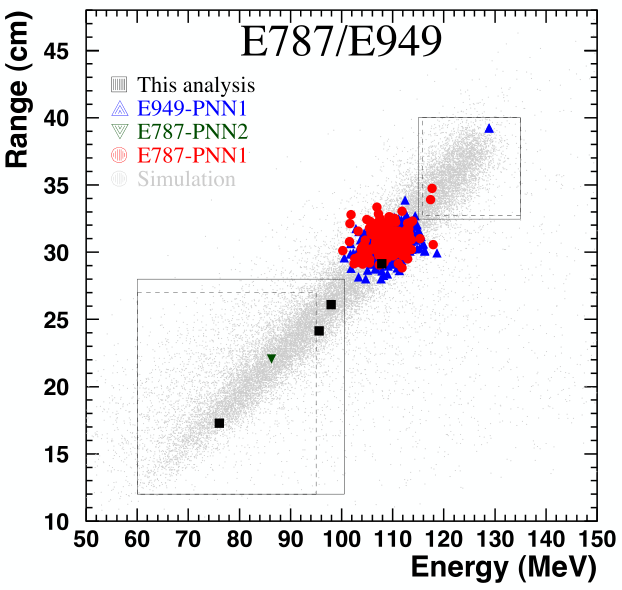
\includegraphics[height=0.6\textheight]{Images/e787ergebnis.png} %Zuschnippeln
            \caption{Ergebnisse von E787a $\rightarrow$ 7 Ereignisse gemessen}
          \end{center}
        \end{figure}
      \end{column}
      \begin{column}{0.5\textwidth}
        \begin{figure}[ht]
          \begin{center}
            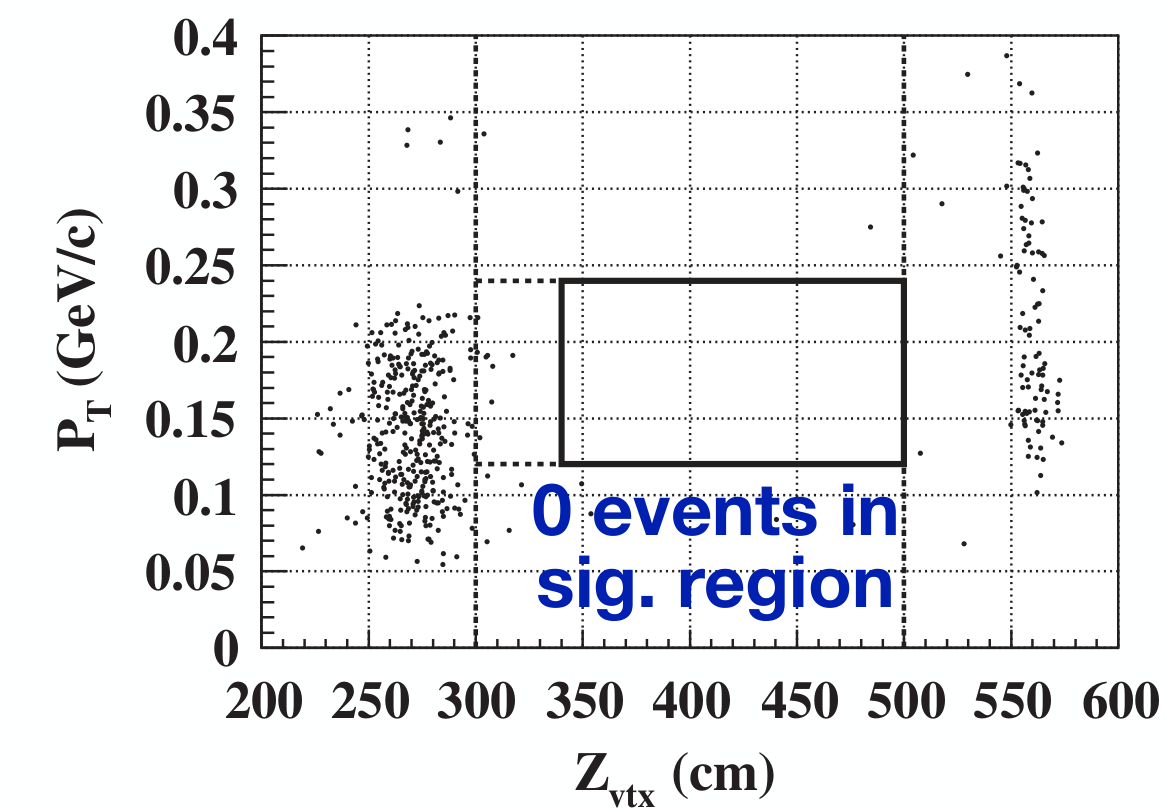
\includegraphics[height=0.6\textheight]{Images/e391aergebnis.png} %Zuschnippeln
            \caption{Ergebnisse von E391a $\rightarrow$ keine Ereignisse gemessen}
          \end{center}
        \end{figure}
      \end{column}
    \end{columns}
\end{frame}

  \subsection{NA62}

  \begin{frame}{NA62 - Übersicht}
    \begin{itemize}
      \setlength{\itemindent}{0.5cm}
      \item[Ziel:] Messung von BR($K^+ \rightarrow \pi^+ \nu \bar{\nu}$)
      \item[Erhofft:] Gleiche Präzision wie Theorie: $\SI{10}{\percent}$
      \item[Benötigt:] $10^{13}$ Zerfälle
    \end{itemize}
    \begin{itemize}
      \item[\rightarrow] Ablehnungsfaktor von $10^{12}$ für andere Zerfälle
      \item Detektorsignatur 'einfach': Einkommendes Kaon zerfällt in einzelnes geladenes Pion
      \item[\rightarrow] Es müssen viele Hintergrundzerfälle gefiltert werden
      \item Detektor ähnlich wie bei NA48
      \item[\rightarrow] Mehr Vetosysteme, genauere Spurdetektoren
    \end{itemize}
  \end{frame}

  \begin{frame}{Detektor}
    \begin{figure}[ht]
      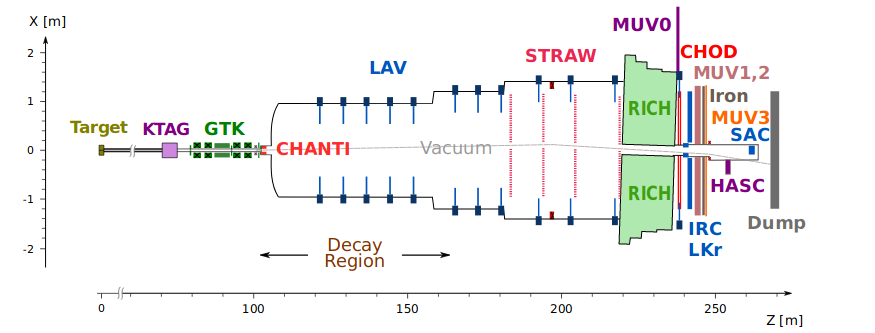
\includegraphics[height=0.75\textheight]{Images/na62detektor.png}
      \caption{Aufbau des genutzten Detektors von NA62}%erinnert ein bissel an NA48
    \end{figure}
  \end{frame}

  \begin{frame}{Kriterienübersicht}
      \begin{columns}[onlytextwidth]
        \begin{column}{0.4\textwidth}
          \begin{figure}[ht]
            \begin{center}
              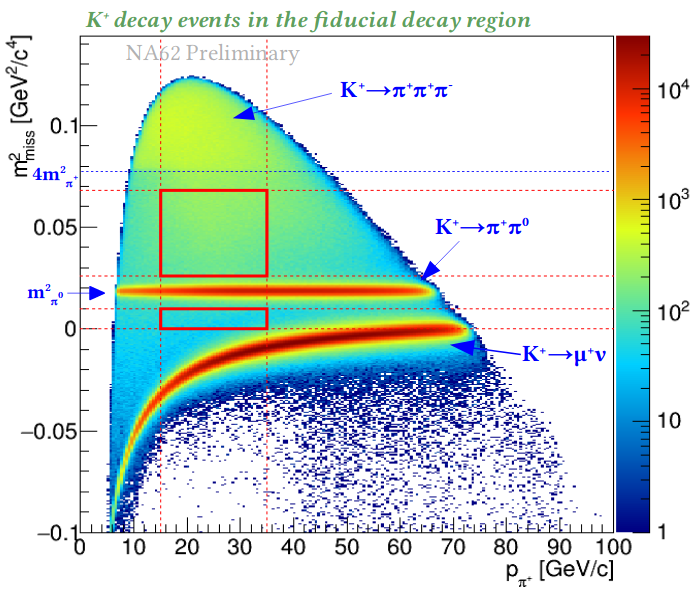
\includegraphics[height=0.8\textheight]{Images/na62decayregion.png} %Zuschnippeln
              \caption{Darstellung der Signalselektion}
            \end{center}
          \end{figure}
        \end{column}
        \begin{column}{0.5\textwidth}
          Übersicht über Kriterien:
          \begin{itemize}
            \item Einzelne Spur im Detektor
            \item $\pi⁺$-Identifikation
            \item $\gamma$-Ausschluss
            \item Multispur-Ausschluss
          \end{itemize}
        \end{column}
      \end{columns}
  \end{frame}

  \begin{frame}{Ergebnis der 2016er Daten}
    \begin{columns}[onlytextwidth]
      \begin{column}{0.4\textwidth}
        \begin{figure}[ht]
          \begin{center}
            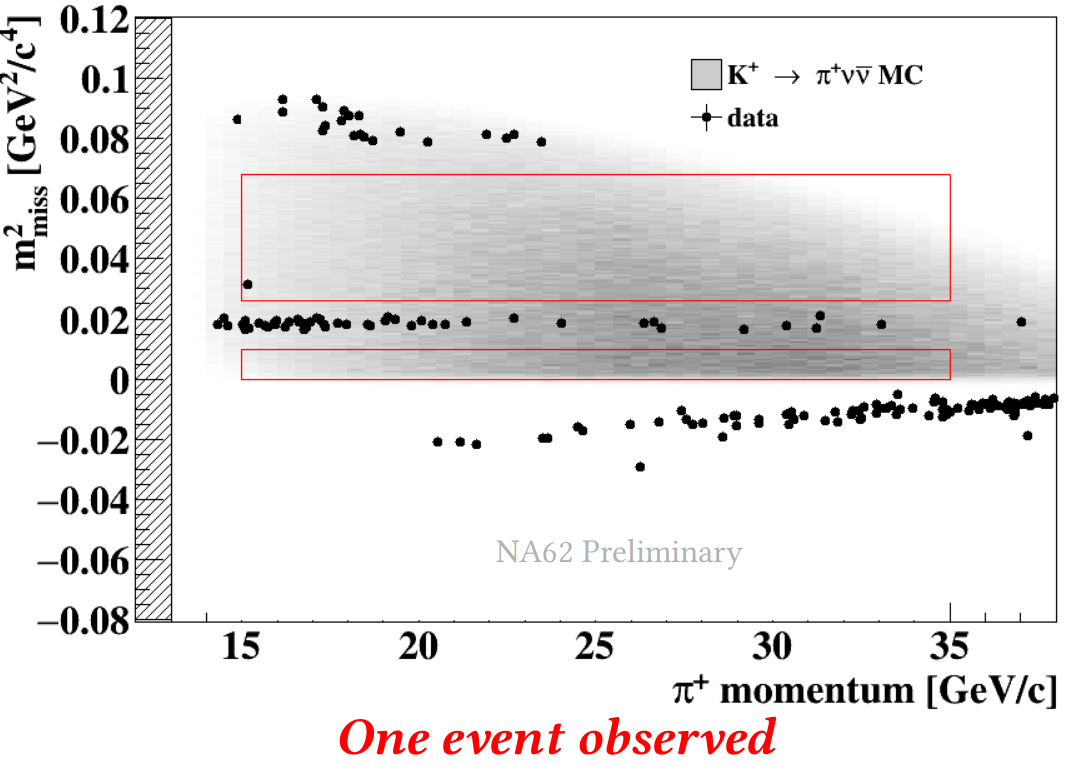
\includegraphics[width=0.9\textwidth]{Images/na622016.png} %Zuschnippeln
            \caption{Resultat der Messungen}
          \end{center}
        \end{figure}
      \end{column}
      \begin{column}{0.5\textwidth}
        Neue Ergebnisse:
        \begin{align*}
          BR(K^+ \rightarrow \pi^+ \nu \bar{\nu}) &< 11 \times 10^{-10} @\, \SI{90}{\percent} CL \\
          BR(K^+ \rightarrow \pi^+ \nu \bar{\nu}) &< 14 \times 10^{-10} @\, \SI{95}{\percent} CL
        \end{align*}
        \begin{itemize}
          \item[\rightarrow] Ergebnisse sind mit SM kompatibel
        \end{itemize}
        Vergleich:
        \begin{align*}
          \symup{Theorie: BR}(K^+ \rightarrow \pi^+ \nu \bar{\nu})     &=  (8.4\pm1.0) \times 10^{-11} \\
        \end{align*}
      \end{column}
    \end{columns}
  \end{frame}

  \subsection{KOTO}

  \begin{frame}{Das KOTO-Experiment}
    \begin{columns}[onlytextwidth]
      \begin{column}{0.4\textwidth}
        \begin{figure}[ht]
          \begin{center}
            
\includegraphics[width=0.9\textwidth]{Images/jparclogo.png}
          \end{center}
        \end{figure}
      \end{column}
      \begin{column}{0.5\textwidth}
        \begin{itemize}
          \item KOTO: K0 at Tokai
          \item Experiment am J-PARC (Japan Proton Accelerator Research Complex)
          \item[\rightarrow] Nutzung des high intensity proton beams ($\SI{30}{\giga\electronvolt}$) des J-PARC
          \item Ähnlicher Zerfall wie NA62: $K_L \rightarrow \pi^0 \nu \bar{\nu}$
          \item[\rightarrow] Wurde von E391a auf $< 2.6 \times 10^{-8} @\, \SI{90}{\percent}$ beschränkt
          %E391a Experiment am J-PArc
          \item Außerdem: $K_L \rightarrow \pi^0 \Chi^0$
          \item[\rightarrow] $\Chi^0$ unsichtbares leichtes Bosonm, mit Masse $\SI{135}{\mega\electronvolt}$
        \end{itemize}
      \end{column}
    \end{columns}
  \end{frame}

  \begin{frame}{Detektor}
    \begin{figure}[ht]
      \begin{center}
        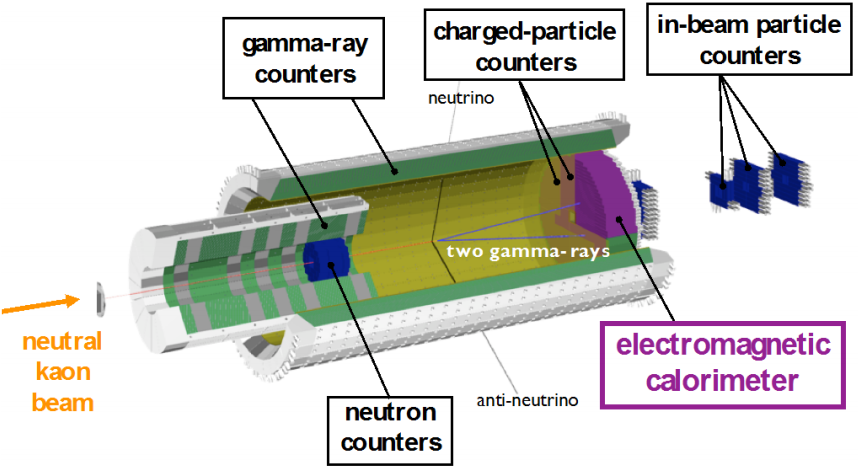
\includegraphics[height=0.8\textheight]{Images/jparcdetektor.png}
        \caption{Schema des KOTO-Detektors} %Ähnliches Schema wie vorher, hier detektion der photonen aus pi^0 zerfall
      \end{center}
    \end{figure}
  \end{frame}

  \begin{frame}
    \begin{columns}[onlytextwidth]
      \begin{column}{0.4\textwidth}
        \begin{figure}[ht]
          \begin{center}
            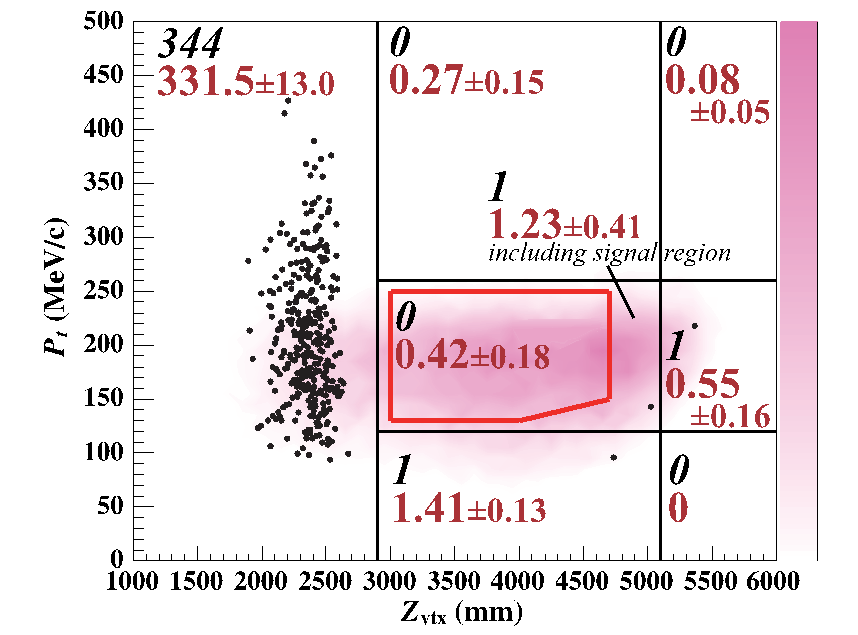
\includegraphics[width=0.9\textwidth]{Images/jparcergebnis.png}
            \caption{Analyse der KOTO-Daten aus 2015} %Es wurde kein Zerfall beobachtet
          \end{center}
        \end{figure}
      \end{column}
      \begin{column}{0.5\textwidth}
        \begin{itemize}
          \item Vorherige Sensitivität auf $K_L \rightarrow \pi^0 \nu \bar{\nu}$ um Größenordnung verbessert:
          \item[\rightarrow] Neue obere schranke von $3.0 \times 10^{-9} @\, \SI{90}{\percent} CL$
          \item[\rightarrow] SM-Vorhersage von $(3.00\pm0.30) \times 10^{-11}$
          \item Vorherige Sensitivität auf $K_L \rightarrow \pi^0 \Chi^0$ verbessert:
          \item[\rightarrow] Neue obere schranke von $2.4 \times 10^{-9} @\, \SI{90}{\percent} CL$
        \end{itemize}
      \end{column}
    \end{columns}
  \end{frame}
  %https://journals.aps.org/prl/abstract/10.1103/PhysRevLett.122.021802

  \subsection{Weitere Experimente}

  \begin{frame}{Weitere Experimente}
    KLOE II:
    \begin{itemize}
      \item Experiment am DA$\upphi$NE-Bechleuniger am INFN Frascate National Laboratory
      \item $e^+e^-$-Beschleuniger
      \item[\rightarrow] Operiert an Massenresonanz des $\upphi$-Mesons @ $\SI{1019}{\mega\electronvolt}$
      \item[\rightarrow] $\upphi$ fast in Ruhe
      \item[\rightarrow] Zerfall in $\SI{49}{\percent}$ in $K^+K^-$ und $\SI{34}{\percent}$ in $K_S K_L$
      \item Messung von $V_{us}$, Untersuchung von CP und CPT diskreten Symmetrien und Dekohärenz von Kaonverschränkung durch KLOE
      \item[\rightarrow] KLOE II soll präzisere Daten liefern
    \end{itemize}
  \end{frame}

  \begin{frame}
    KLEVER:
    \begin{itemize}
      \item Nachfolger/ Zukunft von NA62
      \item Präzisere Messung von BR($K \rightarrow \pi \nu \bar{\nu}$)
      \item Wichtig beide Zerfallsmoden zu vermessen %K+ KL
      \item[\rightarrow] Unterschiedliche Beeinflussung durch verschiedene Modelle neuer Physik
      \item Start der Datennahme im Jahr 2026
      \item Vetomechanismen ähnlich zu KOTO
      \item Upgrade der Strahlproduktionen und Detektion im Vergleich zu NA62
    \end{itemize}
  \end{frame}


















%\section{Kaptel 2}
  %\begin{frame}{Folie 2.1}
    %Text
  %\end{frame}

\end{document}
